% LaTeX source for ``การเรียนรู้ของเครื่องสำหรับเคมีควอนตัม (Machine Learning for Quantum Chemistry)''
% Copyright (c) 2022 รังสิมันต์ เกษแก้ว (Rangsiman Ketkaew).

% License: Creative Commons Attribution-NonCommercial-NoDerivatives 4.0 International (CC BY-NC-ND 4.0)
% https://creativecommons.org/licenses/by-nc-nd/4.0/

%--------------------------
\chapter{เทคนิคการเขียนโมเดล TensorFlow}
\label{ch:coding_tf}
%--------------------------

TensorFlow ถือได้ว่าเป็นไลบรารี่ Neural Network ที่ได้รับความนิยมมากที่สุดในโลกก็ว่าได้ ด้วยฟังก์ชันและโมเดลที่มีให้เลือกใช้งานได้หลากหลาย ทำให้ TensorFlow ถูกนำมาใช้งานในการสร้างและฝึกสอนโมเดล Neural Network ในงานประเภทต่าง ๆ
\idxen{TensorFlow}

%--------------------------
\section{TensorFlow Playground}
\label{sec:tf_playground}
\idxen{TensorFlow!Playground}
%--------------------------

\begin{figure}[H]
    \centering
    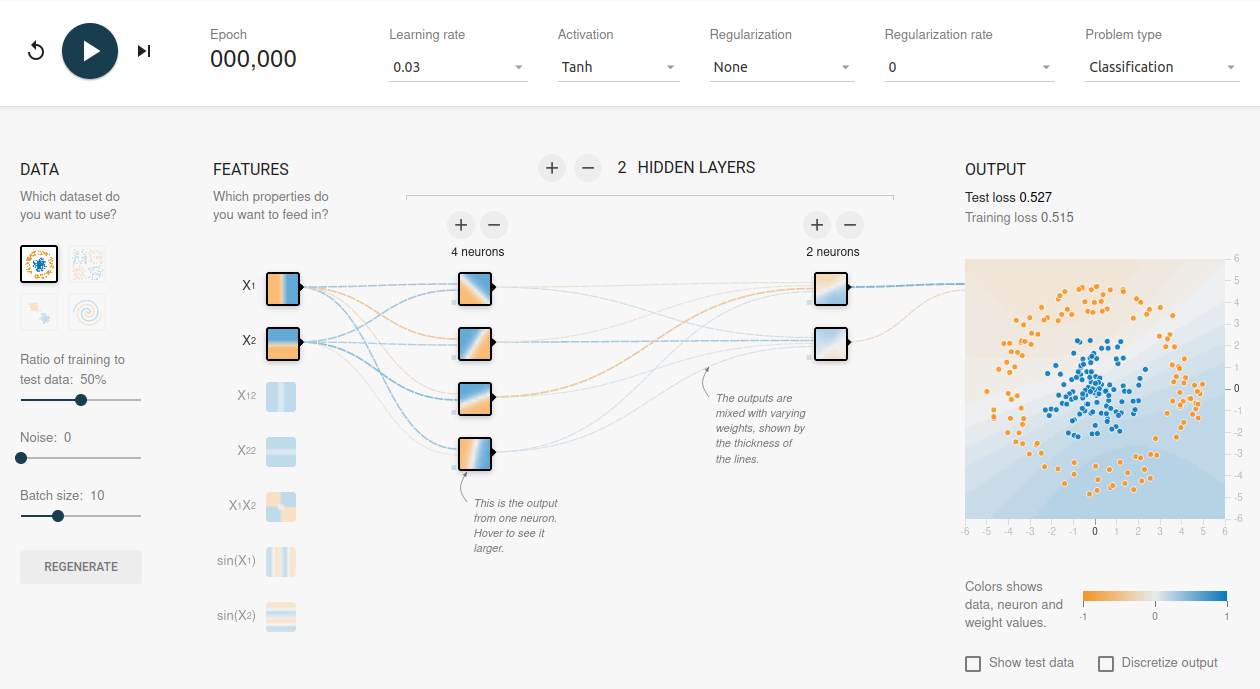
\includegraphics[width=\linewidth]{fig/tf-playground.png}
    \caption{Interface ของ TensorFlow Playground แสดงส่วนควบคุมการตั้งค่า Hyperparameters และการฝึกฝนโมเดล}
    \label{fig:tf_playground}
\end{figure}

TensorFlow Playground คือเว็บไซต์ที่ทาง TensorFlow พัฒนาขึ้นมาเพื่อให้เราเรียนรู้เกี่ยวกับ Neural Network ซึ่งจะมีคอนโซลและเครื่องมือให้เราได้ออกแบบและฝึกฝนโมเดล Neural Network ที่มีขนาดเล็ก ไม่ซับซ้อนมาก แต่ทำงานได้จริง ซึ่งสามารถช่วยให้เราเห็นภาพว่าเกิดอะไรขึ้นบ้างในระหว่างที่มีการฝึกสอนโมเดล ข้อดีของ TensorFlow Playground ก็คือใช้งานได้สะดวกมาก ๆ เพราะสามารถใช้งานผ่านเว็บไซต์ได้เลยและไม่ต้องติดตั้งโปรแกรมอื่น ๆ ให้ยุ่งยาก โดยเข้าใช้งานได้ที่ \url{http://playground.tensorflow.org}

ภาพที่ \ref{fig:tf_playground} แสดงส่วนควบคุมและแสดงผลของการฝึกสอนโมเดล โดยในส่วนด้านบนนั้นจะเป็นคอนโซลในการควบคุมการฝึกสอนโมเดลซึ่งเราสามารถกดเริ่มการฝึกสอนโมเดลได้ทันที และสามารถกดหยุดชั่วคราวได้ด้วย นอกจากนี้เรายังสามารถกำหนด Hyperparameters เช่น Learning Rate, Activation Function, Regularization, Regularization Rate รวมไปถึงประเภทของโจทย์ปัญหาได้ด้วย

ในส่วนทางด้านซ้ายนั้นก็คือการเลือกชุดข้อมูลและการจัดการกับชุดข้อมูล เช่น เราสามารถกำหนดสัดส่วนของการแบ่งชุดข้อมูลได้ โดยค่าเริ่มต้นคือ 50\และยังกำหนด Noise ได้เช่นกัน สำหรับบริเวณตรงกลางนั้นจะเป็นการดีไซน์หรือออกแบบ Nueral Network ที่ต้องการฝึกสอนนั่นเอง เราสามารถเพิ่มหรือลดจำนวนของ Hidden Layer ได้และกำหนดจำนวนของ Node ในแต่ละชั้นได้ด้วยเช่นกัน และทางด้านขวาก็คือการแสดงผลการ Fit ของโมเดลกับข้อมูลซึ่งในกรณีของโจทย์แบบ Classification นั้นจะใช้สีในการแบ่งหรือเป็นเกณฑ์ในการบอกถึงความสามารถในการ Classify ของโมเดล นอกจากนี้ยังมีบอกค่า Test Loss และ Train Loss อีกด้วย

สำหรับคำแนะนำในการใช้งานเพื่อศึกษา Neural Network นั้น ผู้เขียนขอแนะนำให้ผู้อ่านได้ลองเล่น TensorFlow Playground และทำตามดังต่อไปนี้

\begin{enumerate}
    \item เริ่มต้นจากโจทย์ที่ง่ายที่สุดก่อนคือ Classification ของข้อมูลแบบแยก 2 กอง โดยลองลบ Hidden Layer ออกให้หมดและฝึกสอนโมเดลตั้งแต่ไม่มี Hidden Layer แล้วทำการเพิ่มจำนวนของ Hidden Layer ขึ้นเรื่อย ๆ แล้วสังเกตประสิทธิภาพในการ Classify ของโมเดล
    
    \item เมื่อได้ผลลัพธ์การ Classification เป็นที่น่าพอใจแล้วจึงเพิ่มระดับความยากไปที่โจทย์ที่ยากปานกลาง ได้แก่ การแยกข้อมูลแบบ โดนัทล้อมรอบ แล้วตามด้วยการแยกแบบแยกทแยง โดยทำการเพิ่มจำนวน Layer และ Neuron ในแต่ละ Layer 
    
    \item หลังจากที่เราศึกษาถึงผลของจำนวน Layer และ Neuron แล้ว ให้ลองปรับเปลี่ยน Hyperparameter อื่น ๆ เช่น เพิ่ม Feature แล้วให้สังเกตและเปรียบเทียบเอาต์พุต เช่น Loss และจำนวน Epoch ที่ใช้ฝึกสอนโมเดล
    
    \item ศึกษาทำความเข้าใจความหมายขององค์ประกอบต่าง ๆ ของ Neural Network เราอาจจะเพิ่มความท้าทาย เช่น อาจจะจัดแข่งขันพัฒนาโมเดล Neural Network กับเพื่อน โดยกำหนดข้อจำกัดว่า ฝึกสอนโมเดลได้ไม่เกินกี่ Epoch, กำหนด Test Loss ห้ามเกิน 0.05, ให้ใช้ได้มากที่สุด 4 Layer หรือห้ามใช้ ReLU สำหรับ Activation Function เป็นต้น
\end{enumerate}

%--------------------------
\section{การเขียน TensorFlow เบื้องต้น}
\label{sec:tf_basic}
%--------------------------

ตัวอย่างด้านล่างคือการสร้างและฝึกสอนโมเดล Neural Network ด้วย Keras ซึ่งเป็น API ของ TensorFlow จะเห็นได้ว่าเราสามารถเขียนโค้ด Python โดยเริ่มจากการนำเข้าชุดข้อมูลตัวอย่างซึ่งเป็น Mnist มีการแปลงข้อมูล ตามด้วยการสร้าง Neural Network โดยใช้วิธี Sequential กำหนดจำนวนชั้น ประเภทของแต่ละชั้น และมีพารามิเตอร์ที่เราสามารถกำหนดได้ เช่น จำนวน Node หรือ Neuron ของแต่ละชั้นและ Activation Function หลังจากนั้นก็ทำการ Compile โมเดลซึ่งเราสามารถกำหนด Optimizer และ Loss Function ได้ด้วย เมื่อทำการสร้างโมเดลเสร็จแล้ว ก็จะต่อด้วยการฝึกสอนหรือเทรน (Train) โมเดลตามจำนวนรอบ (Epoch) และขั้นตอนสุดท้ายคือการทดสอบโมเดลโดยการทำนายและประเมินผล

\begin{lstlisting}[style=MyPython]
import tensorflow as tf

mnist = tf.keras.datasets.mnist

(x_train, y_train), (x_test, y_test) = mnist.load_data()
x_train, x_test = x_train / 255.0, x_test / 255.0

model = tf.keras.models.Sequential([
  tf.keras.layers.Flatten(input_shape=(28, 28)),
  tf.keras.layers.Dense(128, activation='relu'),
  tf.keras.layers.Dropout(0.2),
  tf.keras.layers.Dense(10, activation='softmax')
])

model.compile(
    optimizer='adam',
    loss='sparse_categorical_crossentropy',
    metrics=['accuracy']
)

model.fit(x_train, y_train, epochs=5)
model.evaluate(x_test, y_test)
\end{lstlisting}

\vspace{1em}

จากโค้ดด้านบนจะเห็นได้เลยว่าจริง ๆ แล้วการเขียนโค้ด ML โดยเฉพาะ Neural Network ไม่ได้ยากเลย เพราะว่าในปัจจุบันเรามีเครื่องมือที่เป็น Framework ต่าง ๆ ที่ถูกพัฒนาขึ้นมาเพื่อช่วยอำนวยความสะดวกให้เรากับในการเขียนโค้ด เพียงแค่ไม่กี่สิบบรรทัดเราก็สามารถสร้างโมเดลได้แล้ว เมื่อเราเข้าใจพื้นฐานในการสร้างโมเดลแล้ว ถ้าหากเราต้องการที่จะต่อยอดโดยการปรับแต่งโมเดลเพื่อให้สามารถจัดการกับงานที่ซับซ้อนขึ้นก็ไม่ใช่เรื่องยาก

%--------------------------
\section{การปรับแต่ง Loss Function}
\label{sec:tf_custom_loss}
%--------------------------

\begin{lstlisting}[style=MyPython]
import tensorflow as tf
import tensorflow.keras.backend as kb
import numpy as np

def custom_loss(y_actual, y_pred):
    custom_loss = tf.experimental.numpy.log10(kb.sum(kb.abs(y_actual - y_pred)) / y_actual.shape[0])
    return custom_loss


x = np.random.randint(1, 4, size=(1000,))
x = np.asarray(x).T

y = x**2
y = np.asarray(y).T
x = x.astype(np.float32)
y = y.astype(np.float32)

keras_model = tf.keras.Sequential(
    [
        tf.keras.layers.Dense(32, activation=tf.nn.relu, input_shape=[1]),
        tf.keras.layers.Dense(32, activation=tf.nn.relu),
        tf.keras.layers.Dense(1),
    ]
)

optimizer = tf.keras.optimizers.RMSprop(0.001)
keras_model.compile(loss=custom_loss, optimizer=optimizer)
keras_model.fit(x, y, batch_size=20, epochs=50)
\end{lstlisting}

%--------------------------
\section{การฝึกสอนโมเดลด้วยการประมวลผลแบบขนานบน GPU หลายตัว}
\label{sec:tf_multi_gpu}
%--------------------------

\begin{lstlisting}[style=MyPython]
import tensorflow as tf

# Use all avialable GPUs
mirrored_strategy = tf.distribute.MirroredStrategy()
# Specify which GPU to be used
mirrored_strategy = tf.distribute.MirroredStrategy(devices=["/gpu:0", "/gpu:1"])

with mirrored_strategy.scope():
    model = tf.keras.Sequential([tf.keras.layers.Dense(1, input_shape=(1,))])

model.compile(loss="mse", optimizer="sgd")

dataset = tf.data.Dataset.from_tensors(([1.0], [1.0])).repeat(100).batch(10)
model.fit(dataset, epochs=2)
model.evaluate(dataset)
\end{lstlisting}

\vspace{1em}

ตัวอย่างด้านบนเป็นการใช้ \pyinline{MirroredStrategy} ซึ่งเป็นวิธีหนึ่งของการทำ Distributed Training ของ TensorFlow โดยเราทำการสร้าง Scope ขึ้นมาก่อน โดยในโค้ดด้านบนเราสร้าง \pyinline{mirrored_strategy} ซึ่งเราสามารถเลือก GPU ที่ต้องการใช้ในการฝึกสอนโมเดลได้ด้วย หลังจากนั้นก็ใช้ฟังก์ชัน \pyinline{with} สำหรับทำการกำหนด Scope และภายในฟังก์ชันนี้เราก็ทำการสร้าง Neural Network ขึ้นมา หลังจากนั้นก็ทำการคอมไพล์โมเดลซึ่งสามารถกำหนดให้อยู่นอก Scope ได้แล้วก็ทำการฝึกสอนโมเดลโดยใช้วิธี \pyinline{fit} ตามปกติ
